\documentclass{Resources/netsci-project}


% :::~ This is the configuration for the bibliography. DO NOT CHANGE
\usepackage[
    backend=biber,
    style=authoryear,
    natbib=false,
    maxcitenames=2,
    minbibnames=1, maxbibnames=99, 
    url=false, 
    doi=true,
    ]{biblatex}
    
    
\addbibresource{thesis.bib}

\subjectarea{Blockchain \& Distributed Ledger Technologies}

\begin{document}
\firstpage{1}

\title{Exercise X: Model / Report}
\author{Author1 (Matriculation Number), Author2 (Matriculation Number)}
\course{Course Name}
\school{Faculty of Business, Economics and Informatics}
\date{Date}

\maketitle

\begin{abstract}
%ENTER ABSTRACT TEXT BELOW
\lipsum[1] %%NOTE: \lipsum CREATES FILLER TEXT. DELETE AND REPLACE WITH OWN CONTENT.
\end{abstract}


\section{Introduction}
%ENTER INTRODUCTION TEXT BELOW
\lipsum[2]
\begin{equation} \label{eqRestMass}
E = mc^2
\end{equation}
\lipsum[3]

\section{Theory}
%ENTER THEORY TEXT BELOW
\lipsum[4]

\subsection{Citations}


This is an example of a citation at the end of sentence: \autocite{testcite}.
Now, this is an example of a citation within the text as used in \textcite{testcite}.

This is a citation to an article \parencite{testcite}. Note that this is intended to be the format in a particular case \parencite{boccalettia06}. If the citation is referenced in the text, as in \cite{Arenas2008}, no parentheses are needed. Multiple  citations can be collapsed into a single one \parencite{Dijkstra1974,ms09,g09}. A book is cited like \cite{wad}. Unpublished work, can also be added \parencite{zanettiicse2012}. All the styles can be seen in the bibliography.

\section{Methods}
\subsection{Apparatus}
%ENTER APPARATUS TEXT BELOW
\lipsum[5]
\begin{figure}
    \centering
    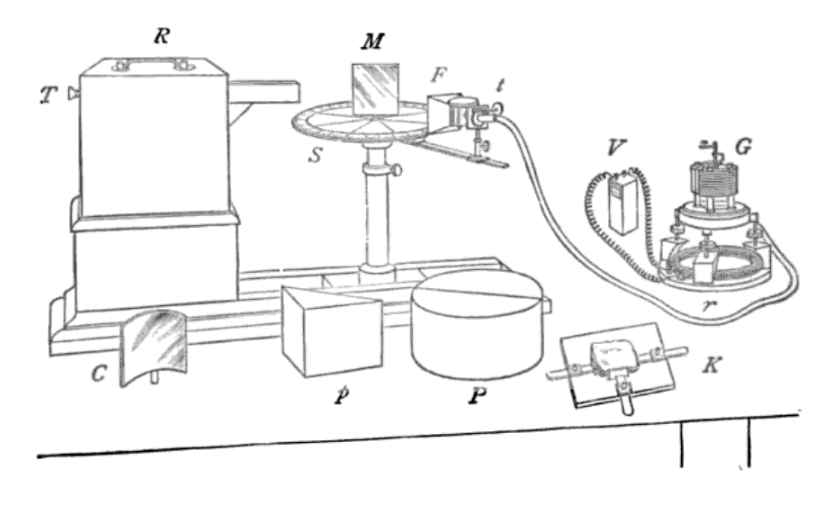
\includegraphics[width=\linewidth]{Resources/apparatus}
    \caption{Optical apparatus used in my experiment.\cite{reference1}}
    \label{fig:my_label}
\end{figure}

\subsection{Procedure}
%ENTER PROCEDURE TEXT BELOW
\lipsum[6]

\section{Results}
%ENTER RESULTS TEXT (AND FIGURES) BELOW
\lipsum[7]

\section{Discussion}
\subsection{Analysis}
%ENTER ANALYSIS TEXT BELOW
\lipsum[8]
Something to be cited.\cite{reference2}
\lipsum[2]

\subsection{Validation}
%ENTER VALIDATION TEXT BELOW
\lipsum[9]

\section{Conclusion}
%ENTER CONCLUSION TEXT BELOW
\lipsum[10]


\printbibliography

\end{document}
